\subsection{RSS3 \glsfmtfull{GI}}
\label{subsec:GI}

{
    \begin{figure}[tb!]
        \centering
        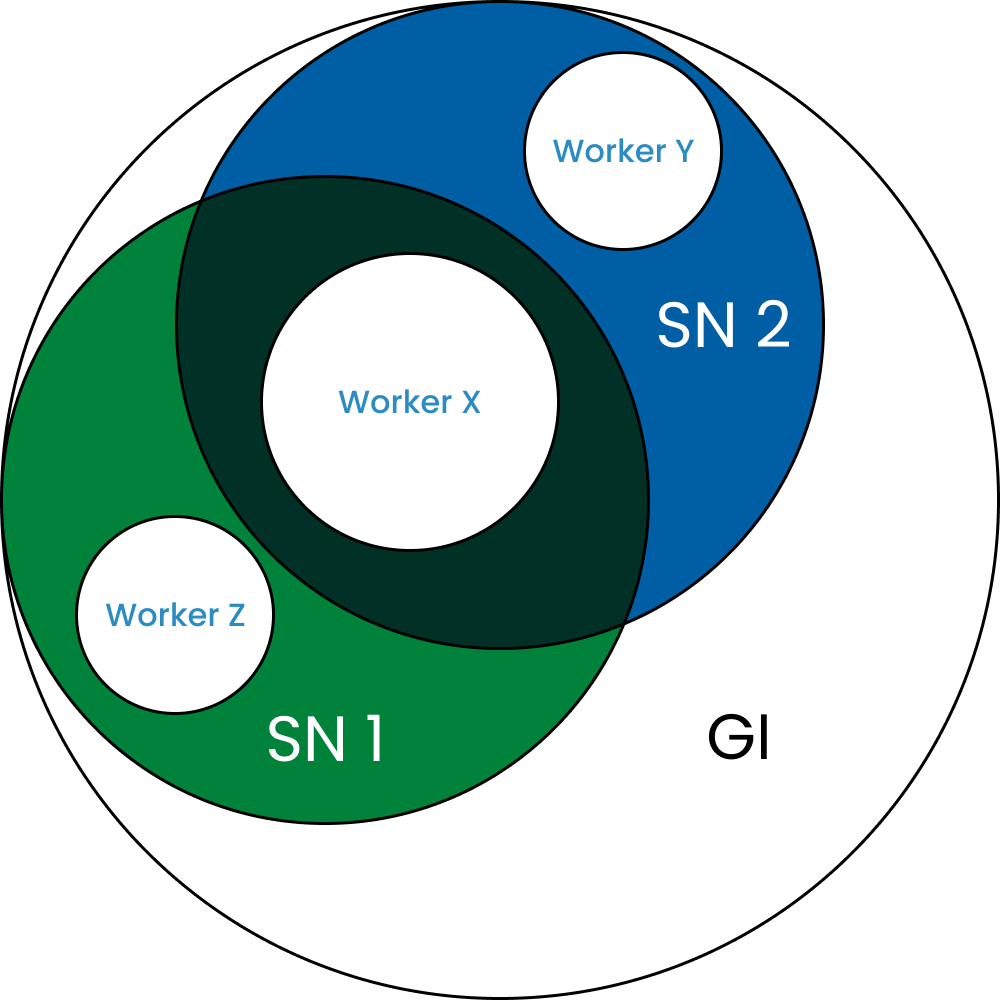
\includegraphics[width=0.7\columnwidth]{figures/GI.png}
        \caption{A Venn diagram illustrating the relationship between the worker, the \glsfmtlong{Node}, and the \glsfmtlong{GI}.}
        \label{fig:GI}
    \end{figure}
}

\glspl{GI} are responsible for facilitating coordination among \glspl{Node} and engaging with the \gls{VSL} and perform critical duties to ensure the \gls{DSL} is robust and reliable.

Given the importance of the \glspl{GI} to the Network, their operation is subject to a set of stringent requirements imposed by the Network.

\subsubsection{Performance Assurance} The routers of \glspl{GI} ensure requests are routed and served with high performance and minimal latency.
The unique architecture of the \gls{DSL} demands \glspl{GI} to be equipped with more computational capabilities to work out the optimal route for processing incoming requests. A request often retrieves \glsfmtlong{OI} from a single \gls{Node} and frequently from a group of \glspl{Node} simultaneously.

\subsubsection{Quality Assurance} The broadcasters and enforcers of \glspl{GI} act as supervisors for \glspl{Node} to ensure the quality of service. The broadcasters constantly monitor all \glspl{Node}' status for irregular behaviors. With the \gls{DSL} being a permissionless Sublayer, the quality needs to be maintained strictly to ensure \glsfmtlong{R3N}'s robustness and reliability.
The enforcers work with the broadcasters and routers to maintain a record of demotion and slashing, and slash a \gls{Node} if it fails to meet the requirements.

\subsubsection{Proof Onchain} The settlers of \glspl{GI} initiate submissions of work records of \glspl{Node} to the \gls{VSL}, and the settlement contract will verify and distribute network rewards.
The payment processors work together with the settlers to ensure that request fees collected are correctly distributed to the corresponding \glspl{Node} and creators.
Additionally, the taxers work out the Network's average tax rate and update the settlement contract on the \gls{VSL}.

\subsection{Reliability Score}

\glspl{GI} route requests to \glspl{Node} based on their information coverage and a \gls{RS}.
The calculation of \reliabilityScore\ is based on a range of factors, including but not limited to the \gls{Node}'s uptime, work, slash records, operation deposit, and staking/trust pool size.
\glspl{Node} with a higher \reliabilityScore\ have an increased likelihood of receiving requests.
